\documentclass[pdf]{beamer}

\mode<presentation>{\usetheme{Warsaw}}

% http://web.mit.edu/rsi/www/pdfs/beamer-tutorial.pdf
% https://rohanverma.net/blog/2017/12/20/setting-up-latex-on-spacemacs/
% begin end CTRL-c CRTL-e

\AtBeginSection[]
{
  \begin{frame}
    \frametitle{Table of Contents}
    \tableofcontents[currentsection, hideothersubsections]
  \end{frame}
}

\title{Automatically responding to customers}
\begin{document}

\begin{frame}
  \titlepage
\end{frame}

\begin{frame}
  \frametitle{Table of Contents}
  \tableofcontents[hideothersubsections]
\end{frame}

\section{Introduction}
\subsection{Research question 1}
\begin{frame}{Existing benchmarks}
  \begin{itemize}
  \item Braun et al.
  \item Snips (next slide)
  \item Burtsev et al.
  \item Botfuel
  \end{itemize}
\end{frame}

\begin{frame}{SNIPS demonstration}
  \begin{center}
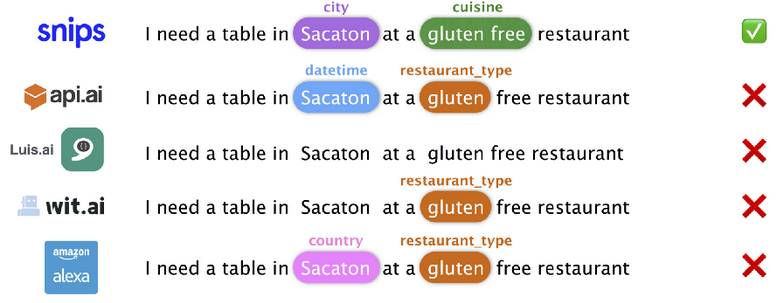
\includegraphics[width=\textwidth]{figures/snips_ner.png}
  \end{center}
\end{frame}

\begin{frame}{SNIPS own benchmark}
  \begin{center}
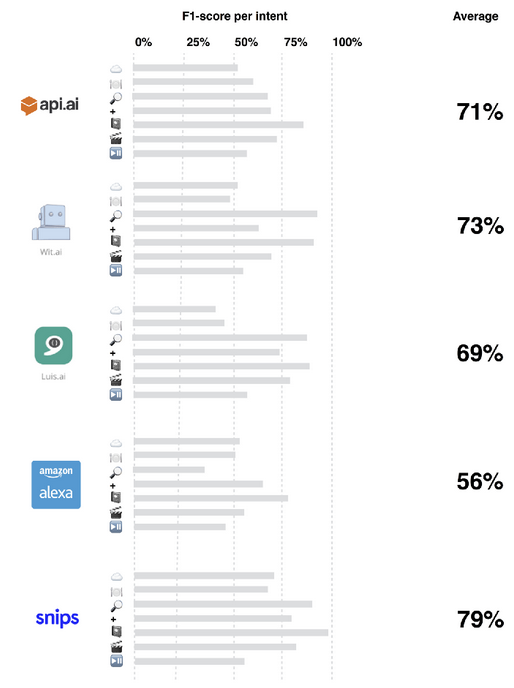
\includegraphics[height=0.85\textheight]{figures/snips_own_benchmark.png}
  \end{center}
\end{frame}

\begin{frame}{Question and goal}
  \begin{itemize}
  \item Can an open-source NLU benchmarking tool be created?
  \item Develop such a tool.
  \end{itemize}
\end{frame}

\subsection{Research question 2}
\begin{frame}{Improving accuracy}
 How hard can it be? 
\end{frame}

\begin{frame}{Question and goal}
  \begin{itemize}
  \item Can accuracy for NLU be increased?
  \item Improve the accuracy
  \end{itemize}
\end{frame}


\section{Preliminaries}
\subsection{Natural language processing}

\subsection{Deep learning}

\section{Benchmarking}
\subsection{Datasets}
\subsection{Systems}
\subsection{Results}

\section{Improving accuracy}

\section{Conclusions}
\subsection{Research question 1}
\begin{frame}{Research question 1}
\end{frame}

\subsection{Research question 2}
\begin{frame}{Research question 2}

\end{frame}
\end{document}
